\documentclass[12pt]{article}\usepackage[]{graphicx}\usepackage[]{color}
%% maxwidth is the original width if it is less than linewidth
%% otherwise use linewidth (to make sure the graphics do not exceed the margin)
\makeatletter
\def\maxwidth{ %
  \ifdim\Gin@nat@width>\linewidth
    \linewidth
  \else
    \Gin@nat@width
  \fi
}
\makeatother

\definecolor{fgcolor}{rgb}{0.345, 0.345, 0.345}
\newcommand{\hlnum}[1]{\textcolor[rgb]{0.686,0.059,0.569}{#1}}%
\newcommand{\hlstr}[1]{\textcolor[rgb]{0.192,0.494,0.8}{#1}}%
\newcommand{\hlcom}[1]{\textcolor[rgb]{0.678,0.584,0.686}{\textit{#1}}}%
\newcommand{\hlopt}[1]{\textcolor[rgb]{0,0,0}{#1}}%
\newcommand{\hlstd}[1]{\textcolor[rgb]{0.345,0.345,0.345}{#1}}%
\newcommand{\hlkwa}[1]{\textcolor[rgb]{0.161,0.373,0.58}{\textbf{#1}}}%
\newcommand{\hlkwb}[1]{\textcolor[rgb]{0.69,0.353,0.396}{#1}}%
\newcommand{\hlkwc}[1]{\textcolor[rgb]{0.333,0.667,0.333}{#1}}%
\newcommand{\hlkwd}[1]{\textcolor[rgb]{0.737,0.353,0.396}{\textbf{#1}}}%
\let\hlipl\hlkwb

\usepackage{framed}
\makeatletter
\newenvironment{kframe}{%
 \def\at@end@of@kframe{}%
 \ifinner\ifhmode%
  \def\at@end@of@kframe{\end{minipage}}%
  \begin{minipage}{\columnwidth}%
 \fi\fi%
 \def\FrameCommand##1{\hskip\@totalleftmargin \hskip-\fboxsep
 \colorbox{shadecolor}{##1}\hskip-\fboxsep
     % There is no \\@totalrightmargin, so:
     \hskip-\linewidth \hskip-\@totalleftmargin \hskip\columnwidth}%
 \MakeFramed {\advance\hsize-\width
   \@totalleftmargin\z@ \linewidth\hsize
   \@setminipage}}%
 {\par\unskip\endMakeFramed%
 \at@end@of@kframe}
\makeatother

\definecolor{shadecolor}{rgb}{.97, .97, .97}
\definecolor{messagecolor}{rgb}{0, 0, 0}
\definecolor{warningcolor}{rgb}{1, 0, 1}
\definecolor{errorcolor}{rgb}{1, 0, 0}
\newenvironment{knitrout}{}{} % an empty environment to be redefined in TeX

\usepackage{alltt}

%% page layout
\textheight 9in 
\textwidth 6.5in
\topmargin -0.5in
\oddsidemargin 0in
\evensidemargin 0in
%\hoffset=-0.5in
\voffset=-0.25in

%% packages
\usepackage{scrtime} % for \thistime (this package MUST be listed first!)
\usepackage{amsmath} % essential for cases environment
\usepackage{amsthm} % for theorems and proofs
\usepackage{amsfonts} % mathbb
\usepackage{graphics,graphicx}
\usepackage{multirow} % fancy tables
\usepackage{wasysym} % circle symbols (including half-filled circles)
\usepackage{enumerate} % fancier enumeration (e.g., a,b,c, ...)
%\usepackage{xcolor}
\usepackage{color}
\newcommand{\de}[1]{{\color{red}{\bfseries DE:} #1}}

%% for solutions to multiple choice questions:
\newcommand{\correct}{{\color{blue}\fbox{\color{red}\checkmark} }}

%% macros
\newcommand{\reals}{\mathbb{R}}
\newcommand{\term}[1]{{\bfseries\slshape #1}}
\newcommand{\Ker}{{\text{Ker}\,}}
\newcommand{\Range}{{\text{Range}\,}}
\newcommand{\diag}{{\text{diag}}}
\newcommand{\alg}{{\text{alg}}}
\newcommand{\geom}{{\text{geom}}}
\newcommand{\norm}[1]{\left\|#1\right\|}
\newcommand{\abs}[1]{\left|#1\right|}
\newcommand{\R}{{\cal R}}
\newcommand{\G}{{\cal G}}
\newcommand{\eps}{\varepsilon}
\newcommand{\B}{\cal B}
\newcommand{\Tinf}{T_\textrm{inf}}
\newcommand{\Shat}{{\hat{S}}}
\newcommand{\Ihat}{{\hat{I}}}
\newcommand{\ie}{\emph{i.e., }}
\newcommand{\eg}{\emph{e.g., }}
\newcommand{\Rlogo}{\protect
\includegraphics[height=2ex,keepaspectratio]{images/Rlogo.pdf}\xspace}
\newcommand{\XPPAUT}{\texttt{XPPAUT}\xspace}
\newcommand{\etal}{\textit{et al}.\xspace}
\newcommand\emphblue[1]{\emph{\color{blue}#1}}

%%%%%%%%%%%%%%%%%%%%%%%%%%%%
%% from feverpreamble.tex %%
%%%%%%%%%%%%%%%%%%%%%%%%%%%%

\usepackage{amssymb,latexsym,amsmath,setspace}
%%\usepackage[colorlinks,linkcolor=blue]{hyperref}
\usepackage[colorlinks=true,allcolors=blue]{hyperref}
%%\usepackage[colorlinks]{hyperref}
\usepackage{xspace}
\usepackage{graphics,graphicx}
\usepackage{subfigure}
\usepackage{lineno}
\usepackage{fancyhdr}
\usepackage[english]{babel}  %% for texi2dvi ~ bug
\usepackage[normalem]{ulem}
\usepackage{tikz} % http://www.texample.net/tikz/examples/tikzdevice-demo/
  % N.B. version 0.6.3 of tikzDevice from Rforge is required!!
%% improve figure caption typsetting:  (see ~/tex/caption.pdf for manual)
\usepackage[footnotesize,bf]{caption}
\usepackage{placeins} % \FloatBarrier

% citation macros
\newcommand{\citen}[1]{\cite{#1}}

% comment macros
\usepackage{color}
\newcommand{\comment}[3]{\textcolor{#1}{\textbf{[#2: }\textit{#3}\textbf{]}}}
\newcommand{\david}[1]{\comment{blue}{DE}{#1}}
\newcommand{\paul}[1]{\comment{cyan}{PA}{#1}}
\newcommand{\ben}[1]{\comment{magenta}{BB}{#1}}
\newcommand{\needref}{{\textcolor{red}{[NEED REF]}}}
\newcommand{\TBD}{{\textcolor{red}{{\bf TBD}}}}
% remove comments
%\renewcommand{\comment}[3]{\relax}
% remove section headings
%\def\subsubsection*#1{\relax\nobreak}

% other macros
\newcommand{\avg}[1]{{\left\langle#1\right\rangle}}
\newcommand{\var}[1]{\textrm{var}\left(#1\right)}
\newcommand{\sem}[1]{\textrm{sem}\left(#1\right)}
\newcommand{\natinf}{{\mathcal I}}
\newcommand{\find}{f_{\textrm{i}}}
\newcommand{\fpop}{f_{\textrm{p}}}
\newcommand{\logit}{\textrm{logit}}
\newcommand{\sign}{\textrm{sign}}
\newcommand{\logistic}{\textrm{logistic}}
\def\AJE{{\it American Journal of Epidemiology\/}}
\newcommand{\code}[1]{{\tt #1}}
\newcommand{\magcode}[1]{{\tt\color{magenta}#1}}
\newcommand{\redcode}[1]{{\tt\color{red}#1}}
\newcommand{\blackcode}[1]{{\tt\color{black}#1}}

%%%%%%%%%%%%%%%%%%%
%% JOURNAL NAMES %%
%%%%%%%%%%%%%%%%%%%
\def\PNAS{PNAS}
\def\JAMA{JAMA}
\def\BMB{{\it Bulletin of Mathematical Biology\/}}

% references
\newcommand{\eref}[1]{Equation~\eqref{E:#1}}
\newcommand{\fref}[1]{Figure~\ref{F:#1}}
\newcommand{\tref}[1]{Table~\ref{T:#1}}
\newcommand{\sref}[1]{\S\ref{S:#1}}
% other macros
\newcommand{{\Reff}}{{\mathcal{R}}_{\rm eff}}
\newcommand{{\Sinit}}{S_{\rm init}}
\newcommand{\supp}{Supplementary Information}
\newcommand{\StoppedHere}{\bigskip\bigskip{\textcolor{red}{\hrule\centerline{\bfseries STOPPED HERE}\hrule}}\bigskip\bigskip}
\newcommand{\colvec}[2]{\begin{pmatrix}#1\\#2\end{pmatrix}}
\newcommand{\diagmat}[3]{\begin{pmatrix}#1&0&0\\0&#2&0\\0&0&#3\end{pmatrix}}

\newcommand{\solution}[1]{{\hfill\break\vspace{-0.5\baselineskip}\break\color{blue}\emph{Solution: }#1}}
\newcommand{\tr}{\text{tr}}

\newcommand{\thickredline}{\bigskip{\color{red}\hrule height 5pt}\bigskip}

%% for assignment 3:
\newtheorem{theorem}{Theorem}
\newtheorem{remark}{Remark}
\newcommand{\openset}{{\mathcal O}}
\newcommand{\C}{{\mathcal C}}

% Journal Names
% -------------
% \def\MNRAS{{\it Mon.\ Not.\ R.\ astr.\ Soc.\/}}
\def\MNRAS{{\it Monthly Notices of the Royal Astronomical Society\/}}
% \def\ApJ{{\it Astrophys.~J.\/}}
\def\ApJ{{\it The Astrophysical Journal\/}}
% \def\Interface{{\it J.\ R.\ Soc.\ Lond.\/ \rm Interface}}
\def\Interface{{\it Journal of the Royal Society of London, \rm Interface}}
% \def\ProcA{{\it Proc.\ R.\ Soc.\ Lond.\/ \rm A}}
\def\ProcA{{\it Proceedings of the Royal Society of London, Series\/ \rm A}}
% \def\ProcB{{\it Proc.\ R.\ Soc.\ Lond.\/ \rm B}}
\def\ProcB{{\it Proceedings of the Royal Society of London, Series\/ \rm B}}
% \def\TransB{{\it Phil.\ Trans.\ R.\ Soc.\ Lond.\/ \rm B}}
\def\TransB{{\it Philosophical Transactions of the Royal Society of London, Series\/ \rm B}}
\def\TREE{{\it Trends in Ecology and Evolution\/}}
% \def\JTB{{\it J.\ theor.\ Biol.\/}}
\def\JTB{{\it Journal of Theoretical Biology\/}}
% \def\BE{{\it Behav.\ Ecol.\/}}
\def\BE{{\it Behavioural Ecology\/}}
% \def\BES{{\it Behav.\ Ecol.\ Sociobiol.\/}}
\def\BES{{\it Behavioural Ecology and Sociobiology\/}}
% \def\BJLS{\it Biol.\ J.\ Linn.\ Soc.\/}}
\def\BJLS{{\it Biological Journal of the Linnean Society\/}}
\def\Nature{{\it Nature\/}}
\def\Science{{\it Science\/}}
\def\Lancet{{\it The Lancet\/}}
\def\LancetID{{\it Lancet Infectious Diseases\/}}
% \def\PNAS{{\it Proc.\ Natl.\ Acad.\ Sci.\ USA}}
\def\PNAS{{\it PNAS -- Proceedings of the National Academy of Sciences of the
U.S.A.}}
\def\PLoSMed{{\it PLoS Medicine\/}}
\def\PLoSCB{{\it PLoS Computational Biology\/}}
\def\EID{{\it Emerging Infectious Diseases\/}}
\def\BMB{{\it Bulletin of Mathematical Biology\/}}
\def\AJE{{\it American Journal of Epidemiology\/}}
\def\TPB{{\it Theoretical Population Biology\/}}
\def\JRSS{{\it Journal of the Royal Statistical Society\/}}
\def\JRSSB{{\it Journal of the Royal Statistical Society Series B\/}}
\def\IRV{{\it Influenza and Other Respiratory Viruses\/}}
\def\JAMA{{\it JAMA -- Journal of the American Medical Association\/}}
\def\JGLR{{\it Journal of Great Lakes Research\/}}
\def\NEJM{{\it New England Journal of Medicine\/}}
\def\JMB{{\it Journal of Mathematical Biology\/}}
\def\Interface{{\it Journal of the Royal Society Interface\/}}
\def\THEE{{\it Theoretical Ecology\/}}
\def\Annals{{\it Annals of Internal Medicine\/}}
\def\PRL{{\it Physical Review Letters\/}}
\def\PRX{{\it Physical Review X\/}}
\def\NAMS{{\it Notices of the American Mathematical Society\/}}

%% underline with smash through:
\newcommand*{\undersmash}[1]{\underline{\smash{#1}}}

%% referring to TeX macros
\newcommand\ttbackslash{{\tt\char`\\}}
\newcommand{\macro}[1]{{\tt\ttbackslash#1}}

%%%%%%%%%%%%%%%%%%%%%%%%%%%%%%%%%%%%%%%%%%%%%%%%%%%%%%%
%% QUESTIONS FOR MATH 4MB/6MB ASSIGNMENT 4.          %%
%% The question texts are used in several documents: %%
%% assignment, solutions, template,                  %%
%% hence it is better to load them from this file.   %%
%%%%%%%%%%%%%%%%%%%%%%%%%%%%%%%%%%%%%%%%%%%%%%%%%%%%%%%

\newcommand{\TSa}{%
You should have received the following data files by e-mail:
\begin{center}
\tt
meas\_uk\_\_lon\_1944-94\_wk.csv\\
meas\_uk\_\_lpl\_1944-94\_wk.csv
\end{center}
These plain text comma-separated-value files list weekly cases of measles (in London and Liverpool, England, from 1944 to 1994).  Depending on which research direction you select, you might receive other files in the same \code{ymdc} (year,month,day,count) format, where the count column might contain cases or deaths, for example.  Write the following \Rlogo functions:
}

\newcommand{\TSai}{%
\magcode{read.ymdc()}.  Read a file in \code{ymdc} format and return a data frame containing these data and including a \code{date} column that has \Rlogo's \magcode{Date} class.  The first (and potentially only) argument to this function should be the \code{filename} of the data file to be read.
}  

\newcommand{\TSaii}{%
\magcode{time.plot()}.  Given a data frame produced using \magcode{read.ymdc()}, display the associated time plot.  The first argument of the function should be the data frame.  Further optional argument(s) should allow the user to smooth the time series with a moving average.  By default, this function should create a new plot but there should be an option to add to an existing plot. Implement this by having a logical \code{add} argument that is false by default (\code{add=FALSE}).  This will allow you to add a smoothed version of the time series on top of the raw data, for example.  The final argument should be the ellipsis (\code{\dots}) so that details such as colour and line style can be passed to the plotting commands used in this function.
}

\newcommand{\TSaiii}{%
\magcode{periodogram()}.  Given a data frame produced using \magcode{read.ymdc()}, display the associated \emph{period   periodogram} (power spectrum as a function of period).  The first argument of the function should be the data frame.  By default, the entire time series should be used, but optional argument(s) should allow the user to specify a time range of interest.  Use \Rlogo's \magcode{spectrum()} function to compute the power spectrum.  Have \code{add} and \code{\dots} arguments as in \magcode{time.plot()}. Note that if \code{v} is a vector containing a time series of interest, you can obtain and plot its \emph{frequency} periodogram as follows.
}

\newcommand{\TSb}{%
Using your functions, make a multi-panel plot that clearly shows the temporal pattern of the time series and how its frequency structure changes over time.  Think carefully about how to make this multi-panel figure as clear as possible for yourselves and your readers.  Describe your figure, explaining what aspects of your figure you feel are puzzling or interesting and may be possible to understand using mechanistic mathematical modelling.  (Repeat this for each of the epidemic time series you are given.)
}

\newcommand{\SEintro}{%
Consider the SI model,
%
\begin{equation}\label{E:SI}
  \frac{dI}{dt} = \beta (N-I) I \,, \qquad I(0)=I_0,
\end{equation}
%
where $\beta$ is the transmission rate, $N$ is the population size and $I(t)$ is the number of infected individuals at time $t$.
}

\newcommand{\SEa}{%
Write an \Rlogo function \magcode{SI.Gillespie()} that uses the Gillespie algorithm to produce a realization of a stochastic process whose mean field dynamics are given by equation \eqref{E:SI} in the limit $N\to\infty$.  Your function should have arguments \code{beta}, \code{N}, \code{I0} and \code{tmax} (the time at which to end the simulation).  You may find it helpful (conceptually) to write equation~\eqref{E:SI} in two-variable form:
  \begin{subequations}
    \begin{align}
      \frac{dS}{dt} &= -\beta S I \,, \qquad S(0)=N-I_0, \\
      \frac{dI}{dt} &= \beta S I \,, \qquad\quad I(0)=I_0.
    \end{align}
  \end{subequations}
Note that there is only one type of event that can occur, so the second part of the Gillespie algorithm (what type of event occurred) is trivial for this model.
}

\long\def\SEb{%
Make a multi-panel plot comparing the deterministic and stochastic dynamics of the SI model for $\beta=1$, $I_0=1$ and $N\in\{32,10^2,10^3,10^4\}$ ($N=32$ is close to $10^{1.5}$).  Each panel should correspond to a different value of $N$ and should show 30 stochastic realizations together with the deterministic solution.

\emph{\underline{Note}:} To make stochastic simulations exactly reproducible use \texttt{\color{magenta}set.seed()}.
}

\newcommand{\Rintro}{%
The natural history of smallpox is shown in \fref{smpxnathist}.  The US Centers for Disease Control and Prevention (CDC) has recently discovered that a group of bioterrorists plans to reintroduce smallpox to the United States.  The CDC has reason to believe that the terrorists are also bioengineers and have successfully altered the virus so that it causes the early rash stage to be twice as long as it was when the virus was last circulating naturally in the 1970s.  Moreover, the existing smallpox vaccine apparently provides no protection against the altered virus.  The CDC wants your opinion on how the alterations to the virus will affect $\R_0$ and the expected final size of an epidemic if the planned attack is successful.
}

\newcommand{\Ra}{%
Construct a compartmental (ODE) smallpox transmission model based on the natural history specified in \fref{smpxnathist}, including vital dynamics but ignoring disease-induced death.
}

\newcommand{\Rb}{%
Use a biological argument to find a formula for $\R_0$.
}

\newcommand{\Rc}{%
Calculate $\R_0$ using the next generation matrix approach.  \emph{\underline{Note}:} Your solution should include $\mathcal F$, $\mathcal V$, $F$, $V$, and $FV^{-1}$, in the most human-friendly form you can find.  However, feel free to use symbolic manipulation software such as \texttt{Maple}, {\slshape Mathematica\/} or \href{http://www.sagemath.org/}{sage} to help with the necessary algebra and matrix computations.
}

\newcommand{\Rd}{%
Based on your model, and $\R_0\sim5$ for unaltered smallpox, what can you say about the difference in $\R_0$ that can be expected for the newly engineered virus vs.\ the original virus?  
    %% (\emph{\underline{Note}:} If you make use of other sources of information, such as books or web sites, cite them appropriately.)
}

\newcommand{\qRe}{% \Re is TeX's real part symbol so can't use it
Write a paragraph that you can imagine e-mailing to the CDC, in which you do your best to answer their questions.
    %% It would be good to get them to find a formula for the growth
    %% rate and then explain how to use their model to estimate R0 for
    %% the new virus after the growth rate has been measured
    %% empirically.  But, the growth rate cannot be found analytically
    %% (the characteristic polynomial has degree 5) so the problem
    %% becomes longer than I want to burden them with right now.
}

\newcommand{\smpxnathistfig}{%
%
\begin{figure}[h]
\begin{center}
\scalebox{1}{
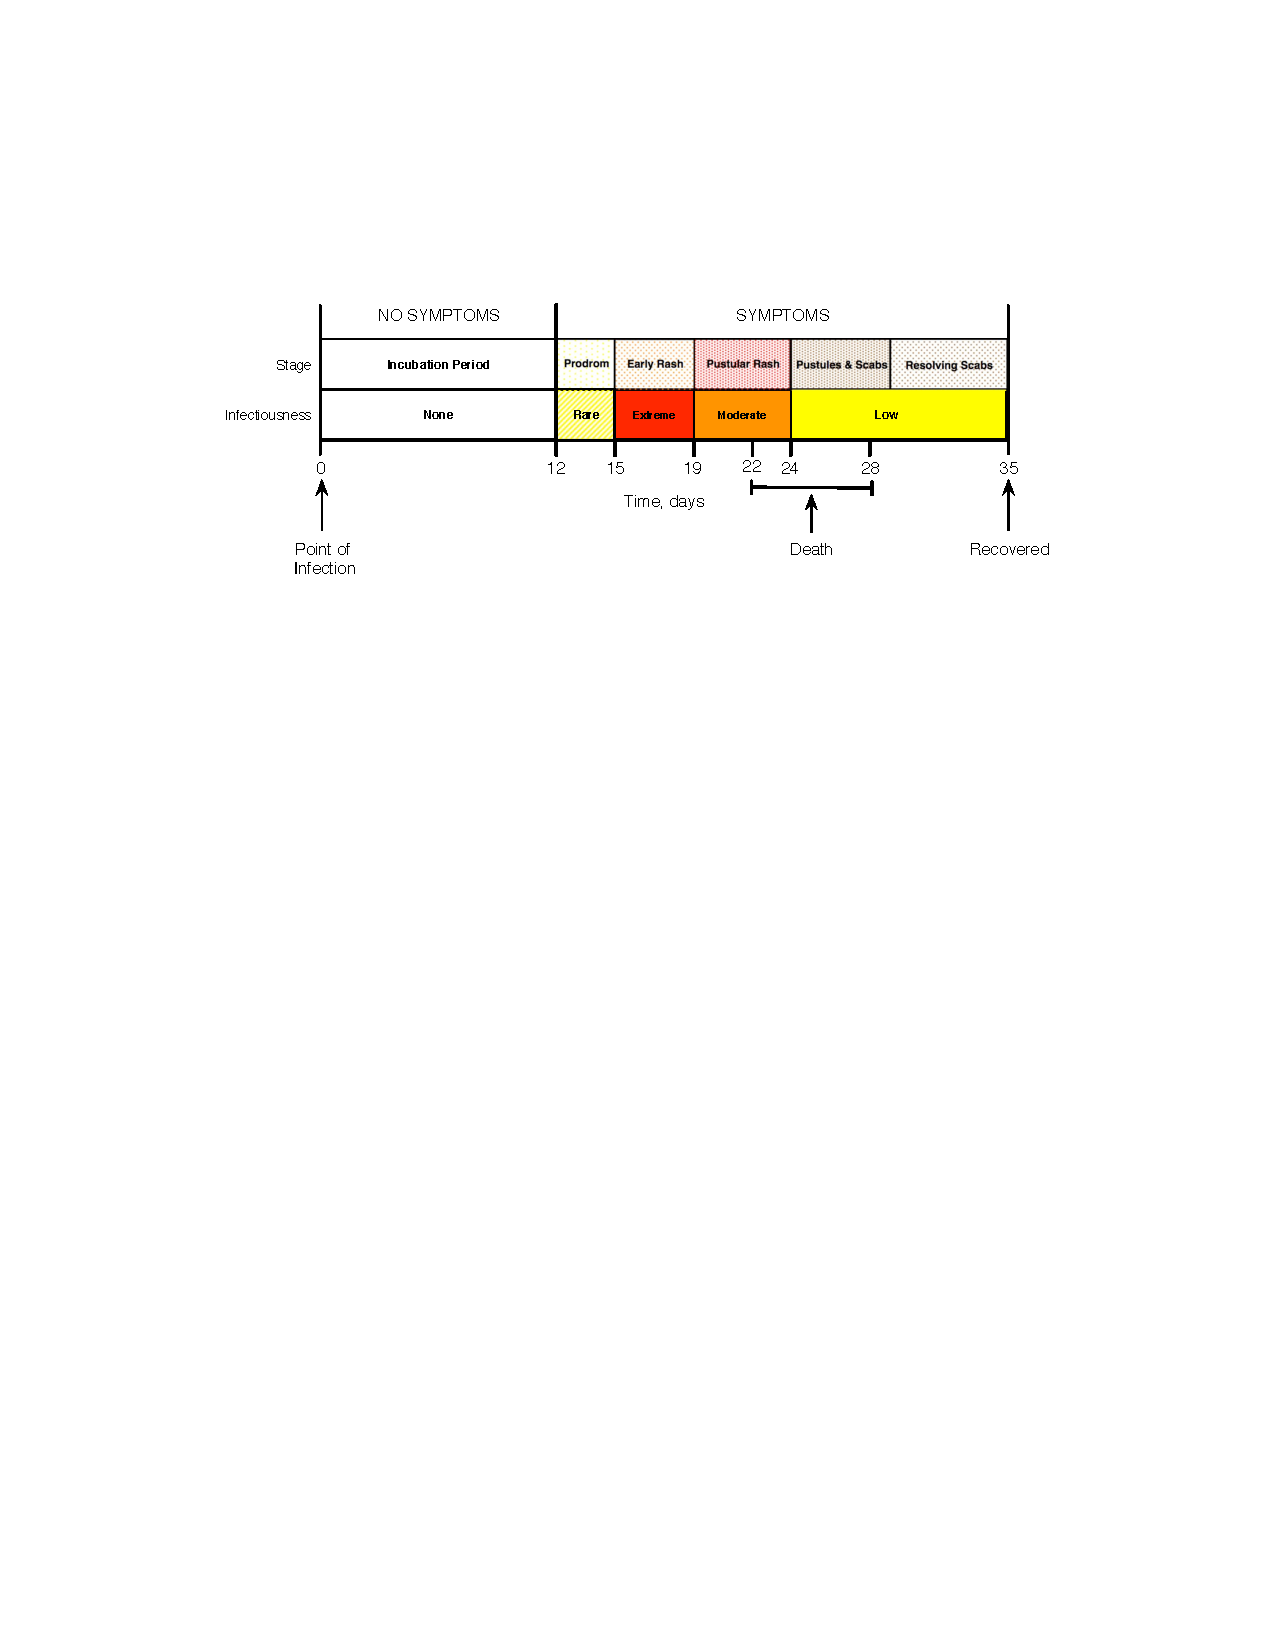
\includegraphics{smpxnathist_p82.pdf}
}
\end{center}
\caption{The natural history of smallpox infection. The prodrom stage begins with fever but the patient is very rarely contagious. Early rash is the most contagious stage, when the rash develops and transforms into bumps. During the pustular rash stage bumps become pustules, which then turn into scabs during the pustules and scabs stage and fall off during the resolving scabs stage. The infected person is contagious until the last scab falls off.  (\emph{This is Figure 3.4 from page 82 of Olga Krylova's 2011 McMaster University PhD thesis.})}
\label{F:smpxnathist}
\end{figure}
%
}

%%\bibliographystyle{vancouver}
%%\bibliography{4mba4_2018}

\newcommand{\BeautifulSolution}{{\color{blue}\begin{proof}{\color{magenta}\dots beautifully clear and concise text to be inserted here\dots}\end{proof}}}

%%%%%%%%%%%%%%%%%%%%%%%%%%%%%%%%%%%
%% FANCY HEADER AND FOOTER STUFF %%
%%%%%%%%%%%%%%%%%%%%%%%%%%%%%%%%%%%
\usepackage{fancyhdr,lastpage}
\pagestyle{fancy}
\fancyhf{} % clear all header and footer parameters
%%%\lhead{Student Name: \theblank{4cm}}
%%%\chead{}
%%%\rhead{Student Number: \theblank{3cm}}
%%%\lfoot{\small\bfseries\ifnum\thepage<\pageref{LastPage}{CONTINUED\\on next page}\else{LAST PAGE}\fi}
\lfoot{}
\cfoot{{\small\bfseries Page \thepage\ of \pageref{LastPage}}}
\rfoot{}
\renewcommand\headrulewidth{0pt} % Removes funny header line
%%%%%%%%%%%%%%%%%%%%%%%%%%%%%%%%%%%
\IfFileExists{upquote.sty}{\usepackage{upquote}}{}
\begin{document}

\begin{center}
{\bf Mathematics 4MB3/6MB3 Mathematical Biology\\
\smallskip
2016 ASSIGNMENT \textcolor{blue}{4}}\\
\medskip
\underline{\emph{Group Name}}: \texttt{{\color{blue}The Infective Collective}}\\
\medskip
\underline{\emph{Group Members}}: {\color{blue}Aurora Basinski-Ferris, Michael Chong, Daniel Park, Daniel Presta}
\end{center}

\bigskip
\noindent
\textcolor{blue}{This assignment was due on Wednesday 14 March 2018 at 11:30am.}

\bigskip

\section{Time Series analysis of Recurrent Epidemics}

\begin{enumerate}[(a)]

\item \TSa

\begin{enumerate}[(i)]

\item \TSai

{\color{blue}{Below, we create a function which returns a data frame with a date column and an associated data column. This is done by mutating the initial data frame from the csv file. We string together the year, month, and day that are originally in three separate columns, and then make this string part of the Date class.}}
\begin{knitrout}
\definecolor{shadecolor}{rgb}{0.969, 0.969, 0.969}\color{fgcolor}\begin{kframe}
\begin{alltt}
\hlkwd{library}\hlstd{(tidyverse)} \hlcom{#load necessary packages}
\hlkwd{library}\hlstd{(stringr)}
\hlstd{read.ymdc} \hlkwb{<-} \hlkwa{function}\hlstd{(}\hlkwc{filename}\hlstd{) \{}
  \hlstd{df}\hlkwb{<-} \hlkwd{read.csv}\hlstd{(filename,} \hlkwc{skip}\hlstd{=}\hlnum{6}\hlstd{)} \hlcom{#skip 6 because 6 lines }
  \hlcom{#at top of csv file that aren't data}
  \hlstd{df} \hlopt \hlkwd{mutate}\hlstd{(}\hlkwc{date}\hlstd{=} \hlkwd{as.Date}\hlstd{(}\hlkwd{str_c}\hlstd{(year,month,day,}\hlkwc{sep}\hlstd{=}\hlstr{'-'}\hlstd{)))} \hlopt
    \hlkwd{select}\hlstd{(}\hlopt{-}\hlstd{year,}\hlopt{-}\hlstd{month,}\hlopt{-}\hlstd{day)}
\hlstd{\}}
\end{alltt}
\end{kframe}
\end{knitrout}

\item \TSaii

{\color{blue}{Next, we create a function which produces a moving average time plot. We modify the data frame that the user supplies when calling the function such that each row is an average of the following s rows and the prior s rows (if s is the value that the user specifies to compute the moving average over). We also delete the first s rows and the last s rows. By default, the plot is separate from any previous plots that the user may have created, but you may add the plot to an existing plot by inputting `TRUE' in the third argument of the function.}}
\begin{knitrout}
\definecolor{shadecolor}{rgb}{0.969, 0.969, 0.969}\color{fgcolor}\begin{kframe}
\begin{alltt}
\hlstd{time.plot} \hlkwb{<-} \hlkwa{function}\hlstd{(}\hlkwc{df}\hlstd{,} \hlkwc{s}\hlstd{,} \hlkwc{add}\hlstd{=}\hlnum{FALSE}\hlstd{,} \hlkwc{...}\hlstd{) \{}
  \hlstd{df2} \hlkwb{<-} \hlstd{df}
  \hlkwa{for} \hlstd{(i} \hlkwa{in} \hlstd{(s}\hlopt{+}\hlnum{1}\hlstd{)}\hlopt{:}\hlstd{(}\hlkwd{nrow}\hlstd{(df2)}\hlopt{-}\hlstd{s)) \{}
  \hlstd{df2}\hlopt{$}\hlstd{cases[i]}\hlkwb{<-}\hlkwd{mean}\hlstd{(df}\hlopt{$}\hlstd{cases[(i}\hlopt{-}\hlstd{s)}\hlopt{:}\hlstd{(i}\hlopt{+}\hlstd{s)])}
  \hlstd{\}}
  \hlstd{df2}\hlopt{$}\hlstd{cases[}\hlnum{1}\hlopt{:}\hlstd{s]}\hlkwb{<-}\hlnum{NA}
  \hlstd{df2}\hlopt{$}\hlstd{cases[(}\hlkwd{nrow}\hlstd{(df2)}\hlopt{-}\hlstd{s)}\hlopt{:}\hlstd{(}\hlkwd{nrow}\hlstd{(df2))]} \hlkwb{<-}\hlnum{NA}

  \hlkwa{if}\hlstd{(add) \{}
    \hlkwd{lines}\hlstd{(df2}\hlopt{$}\hlstd{date,df2}\hlopt{$}\hlstd{cases, ...)}
  \hlstd{\}} \hlkwa{else} \hlstd{\{}
  \hlkwd{plot}\hlstd{(df2}\hlopt{$}\hlstd{date, df2}\hlopt{$}\hlstd{cases,}\hlkwc{type}\hlstd{=}\hlstr{"l"}\hlstd{, ...)}
  \hlstd{\}}
\hlstd{\}}
\end{alltt}
\end{kframe}
\end{knitrout}

\item \TSaiii

{\color{blue}{Finally, we create a function which produces a periodogram on a specific date range of a time series. By default, we have that the begin date is the beginning of the time series and the end date is the end of the time series. However, these can be modified by the user. The function filters the data frame to only include the date range specified by the user. Then it performs a periodogram on that filtered data frame using the commands given in the assignment. Similar to the time.plot function, by default, the plot is separate from any previous plots the user may have created, but the plot may be added to an existing plot by specifiying `TRUE' in the fourth argument of the function.}}
\begin{knitrout}
\definecolor{shadecolor}{rgb}{0.969, 0.969, 0.969}\color{fgcolor}\begin{kframe}
\begin{alltt}
\hlstd{periodogram} \hlkwb{<-}\hlkwa{function}\hlstd{(}\hlkwc{df}\hlstd{,}
                       \hlkwc{start.date}\hlstd{=}\hlkwd{as.Date}\hlstd{(df}\hlopt{$}\hlstd{date[}\hlnum{1}\hlstd{]),}
                       \hlkwc{end.date}\hlstd{=}\hlkwd{as.Date}\hlstd{(df}\hlopt{$}\hlstd{date[}\hlkwd{nrow}\hlstd{(df)]),}
                       \hlkwc{add}\hlstd{=}\hlnum{FALSE}\hlstd{,} \hlkwc{...}\hlstd{) \{}
   \hlstd{df} \hlkwb{<-} \hlstd{df} \hlopt
    \hlkwd{filter}\hlstd{(date} \hlopt{>=} \hlstd{start.date} \hlopt{&} \hlstd{date}\hlopt{<=}\hlstd{end.date)}

\hlstd{s} \hlkwb{<-} \hlkwd{spectrum}\hlstd{(df}\hlopt{$}\hlstd{cases,} \hlkwc{plot} \hlstd{=} \hlnum{FALSE}\hlstd{)}
\hlkwd{plot}\hlstd{((s}\hlopt{$}\hlstd{freq)}\hlopt{^}\hlstd{(}\hlopt{-}\hlnum{1}\hlstd{), s}\hlopt{$}\hlstd{spec,} \hlkwc{type}\hlstd{=}\hlstr{'l'}\hlstd{, ...)}
\hlstd{\}}
\end{alltt}
\end{kframe}
\end{knitrout}

\end{enumerate}

\item \TSb

{\color{blue}{First, we perform analysis on the London time series. Our first step is to plot the time series, as well as a plot smoothed by a 10 week moving average. This smoothed data helps us identify areas of the time series that appear to have similar patterns. Namely, we note that the beginning of the time series until around 1950 appears to have consistent patterns. We also note that the data from around 1950 to 1975 and 1975 until 1994 appear to have similar structure. To investigate these claims, we plot periodograms. Our first periodogram looks at the entire time series (we cut it off at 250 weeks as when we plotted the whole 2500 weeks, we stop seeing patterns after around 200 weeks). This first periodogram tells us that across the whole time series, the most power is at around the 100 week mark, and the next most power is located around the 50 week mark. We note that these roughly correlate to 2 and 1 year cycles. Next, to investigate how these cycles may change over the time series, we plot periodograms for the intervals mentioned earlier which we identified through the initial moving average plot. The plot in the upper right corner shows the periodogram for the period from the beginning of the time series until 1 January 1950. We see that in this time period, the most power is located around the 50 week mark. Next, we plot the time interval from 1 January 1950 until 1 January 1975. Here, we see that the most power is located around the 2 year mark, while there is also a significant amount of power located around the 1 year mark. This tells us that in this period, there are mostly 2 year cycles, with a less significant 1 year cycle. Finally, we look at the end of the time series (from 1 January 1975 until 31 December 1994). In this periodogram, we see that the most power is located around the 140 week mark, with the next most significant power around the 50 week mark. This suggests that in this time period, the most significant cycle is around a three year cycle. However, if we look at the periodogram for the whole time series, we see that that cycle is insignificant overall compared to the 1 year and 2 year cycles. This may be because the three year cycle only appares in the last part of the time series. It also may be because the magnitude of power behind this cycle is much lower than the other cycles in other sections of data.}}
\begin{knitrout}
\definecolor{shadecolor}{rgb}{0.969, 0.969, 0.969}\color{fgcolor}\begin{kframe}
\begin{alltt}
\hlcom{#load london time series using function from 1a(i)}
\hlstd{londondata} \hlkwb{<-} \hlkwd{read.ymdc}\hlstd{(}\hlstr{'meas_uk__lon_1944-94_wk.csv'}\hlstd{)}
\hlkwd{plot}\hlstd{(londondata}\hlopt{$}\hlstd{date, londondata}\hlopt{$}\hlstd{cases,} \hlkwc{xlab}\hlstd{=}\hlstr{"Weeks"}\hlstd{,} \hlkwc{ylab}\hlstd{=}\hlstr{"Incidence"}\hlstd{,}
     \hlkwc{main} \hlstd{=}\hlstr{"10 Week Moving Average Plot of Liverpool Data"}\hlstd{)}
\hlcom{#plot using 10 week moving average using function from 1a(ii)}
\hlkwd{time.plot}\hlstd{(londondata,}\hlnum{10}\hlstd{,}\hlkwc{add}\hlstd{=} \hlnum{TRUE}\hlstd{,} \hlkwc{col}\hlstd{=}\hlstr{'red'}\hlstd{)}
\end{alltt}
\end{kframe}
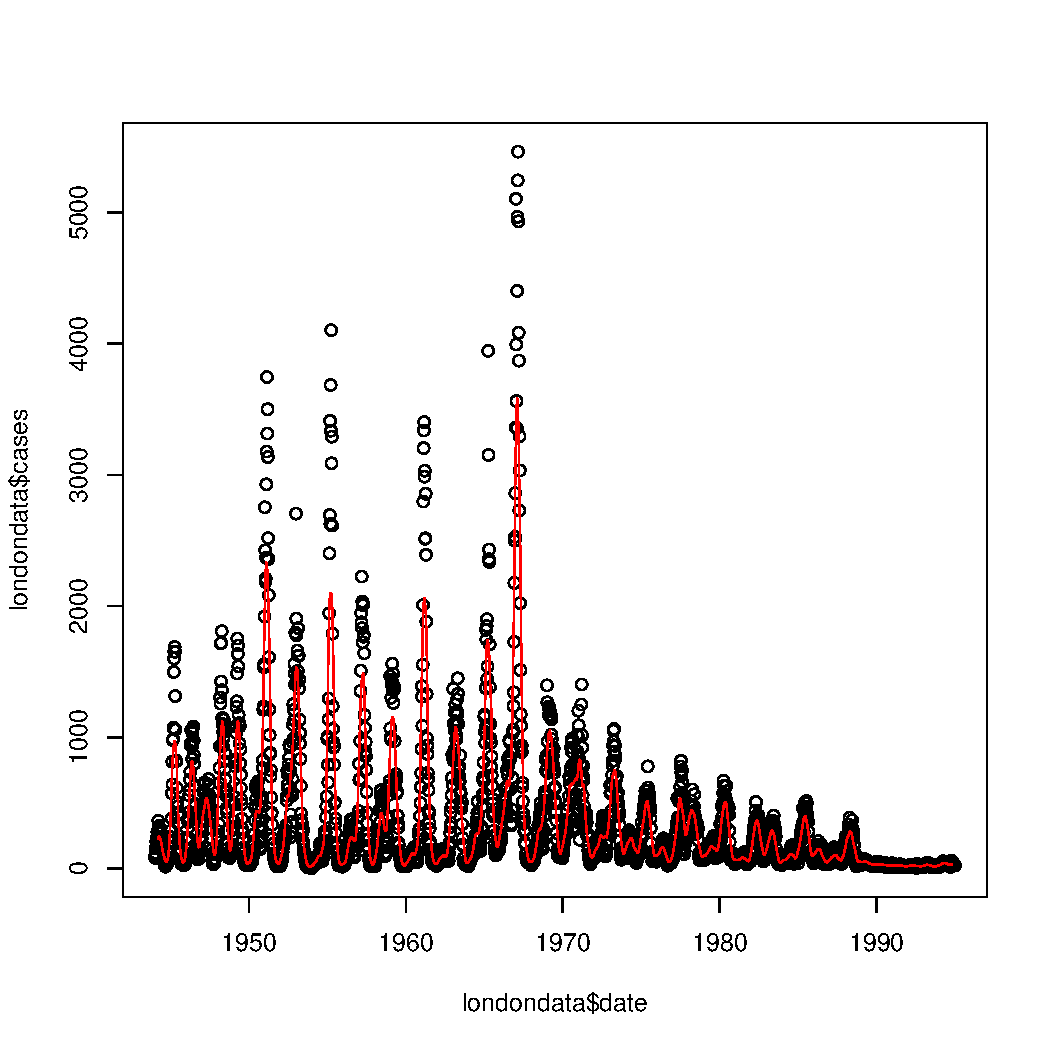
\includegraphics[width=\maxwidth]{figure/unnamed-chunk-4-1} 
\begin{kframe}\begin{alltt}
\hlkwd{par}\hlstd{(}\hlkwc{mfrow}\hlstd{=}\hlkwd{c}\hlstd{(}\hlnum{2}\hlstd{,}\hlnum{2}\hlstd{))} \hlcom{#create multiplot. two columns and two rows}

\hlkwd{periodogram}\hlstd{(londondata,}
            \hlkwc{xlim}\hlstd{=}\hlkwd{c}\hlstd{(}\hlnum{0}\hlstd{,}\hlnum{250}\hlstd{),}
            \hlkwc{main}\hlstd{=}\hlstr{"Entire time series"}\hlstd{,}
            \hlkwc{xlab}\hlstd{=}\hlstr{"Weeks"}\hlstd{,}
            \hlkwc{ylab}\hlstd{=}\hlstr{"Power"}\hlstd{)}

\hlkwd{periodogram}\hlstd{(londondata,}
            \hlkwc{end.date}\hlstd{=}\hlkwd{as.Date}\hlstd{(}\hlstr{'1950-01-01'}\hlstd{),}
            \hlkwc{xlim}\hlstd{=}\hlkwd{c}\hlstd{(}\hlnum{1}\hlstd{,}\hlnum{250}\hlstd{),}
            \hlkwc{main}\hlstd{=}\hlstr{"1944-01-07 to 1950-01-01"}\hlstd{,}
            \hlkwc{xlab}\hlstd{=}\hlstr{"Weeks"}\hlstd{,} \hlkwc{ylab}\hlstd{=}\hlstr{"Power"}\hlstd{)}

\hlkwd{periodogram}\hlstd{(londondata,}
            \hlkwd{as.Date}\hlstd{(}\hlstr{'1950-01-01'}\hlstd{),}
            \hlkwd{as.Date}\hlstd{(}\hlstr{'1975-01-01'}\hlstd{),}
            \hlkwc{xlim}\hlstd{=}\hlkwd{c}\hlstd{(}\hlnum{1}\hlstd{,}\hlnum{250}\hlstd{),}
            \hlkwc{main}\hlstd{=}\hlstr{"1950-01-01 to 1975-01-01"}\hlstd{,}
            \hlkwc{xlab}\hlstd{=}\hlstr{"Weeks"}\hlstd{,} \hlkwc{ylab}\hlstd{=}\hlstr{"Power"}\hlstd{)}

\hlkwd{periodogram}\hlstd{(londondata,}
            \hlkwd{as.Date}\hlstd{(}\hlstr{'1975-01-01'}\hlstd{),}
            \hlkwd{as.Date}\hlstd{(}\hlstr{'1994-12-31'}\hlstd{),}
            \hlkwc{xlim}\hlstd{=}\hlkwd{c}\hlstd{(}\hlnum{1}\hlstd{,}\hlnum{250}\hlstd{),}
            \hlkwc{main}\hlstd{=}\hlstr{"1975-01-01 to 1994-12-31"}\hlstd{,}
            \hlkwc{xlab}\hlstd{=}\hlstr{"Weeks"}\hlstd{,} \hlkwc{ylab}\hlstd{=}\hlstr{"Power"}\hlstd{)}
\end{alltt}
\end{kframe}
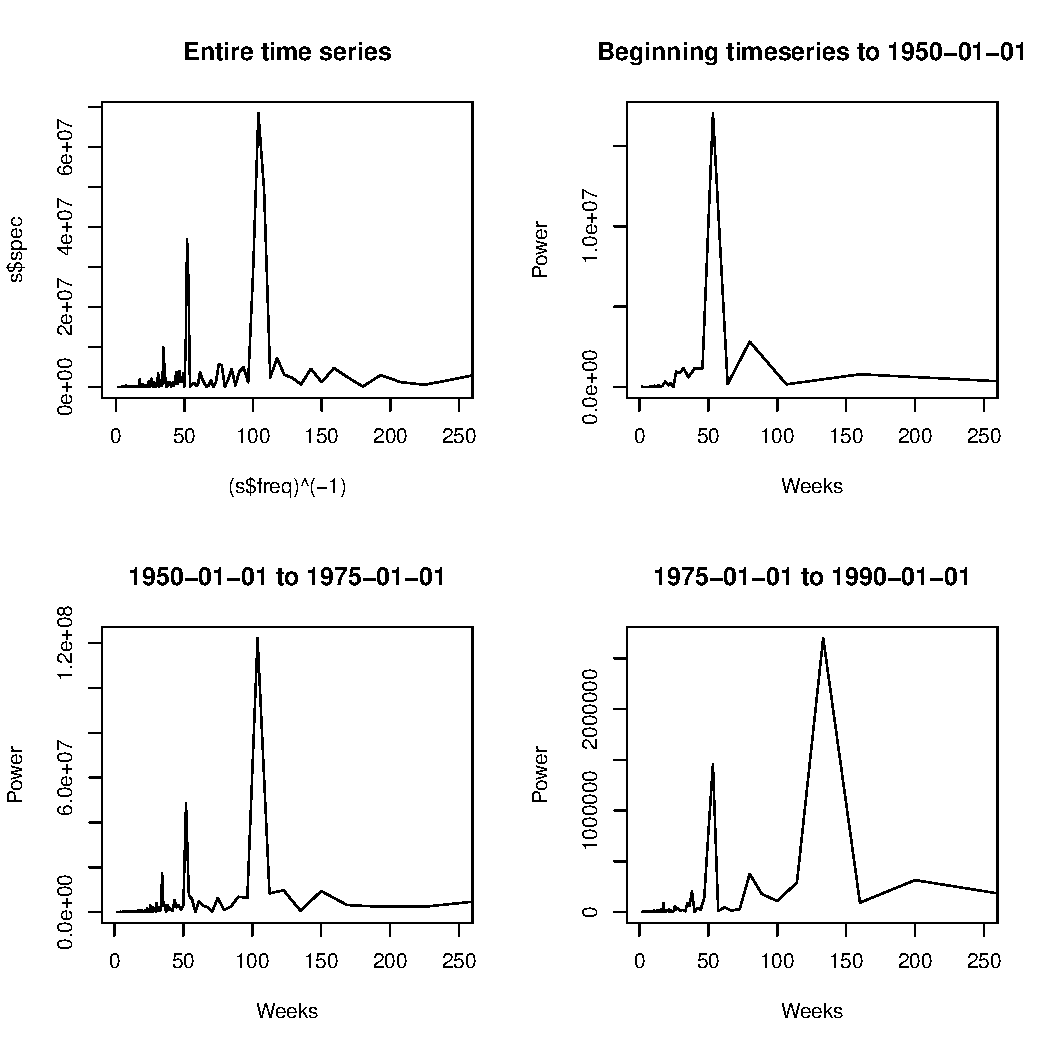
\includegraphics[width=\maxwidth]{figure/unnamed-chunk-4-2} 

\end{knitrout}

{\color{blue}{Next, we perform analysis on the Liverpool time series. Again, our first step is to plot the time series, as well as a plot smoothed by a 10 week moving average. Based on this smoothed data, we identify intervals of interest again, which will be tweaked and investigated with periodograms. These intervals identified are from the beginning of the data set to 1950, from 1950 until just before 1970, and from just before 1970 until the end of the time series. Our first plot is a periodogram of the whole time series. In this plot, we can see that the patterns across the whole time series aren't as clear as in the London data series. However, there appear to be strong 1 year and 2 year cycles despite some other less significant cycles present. We then investigate the intervals of interest which we identified through visual patterns in the moving average plot. First, we looked at the time interval from the beginning of the time series until 1 January 1950. The periodogram for this time revealed that the the strongest cycle in this time was around 1 year. Next, we found that the strongest cycle in the time period from 1 January 1950 until 1 January 1968 was two years. However, there was also a weak 1 year cycle present. Finally, in the time period from 1 January 1968 until 31 December 1994, we find that the most power is around the 130 week mark. However, there is also a significant amount of power around the 50 week mark.}}
\begin{knitrout}
\definecolor{shadecolor}{rgb}{0.969, 0.969, 0.969}\color{fgcolor}\begin{kframe}
\begin{alltt}
\hlcom{#Perform analysis on the lpl time series}
\hlcom{#load liverpool time series}
\hlstd{lpldata}\hlkwb{<-}\hlkwd{read.ymdc}\hlstd{(}\hlstr{'meas_uk__lpl_1944-94_wk.csv'}\hlstd{)}
\hlkwd{plot}\hlstd{(lpldata}\hlopt{$}\hlstd{date, lpldata}\hlopt{$}\hlstd{cases,} \hlkwc{xlab}\hlstd{=}\hlstr{"Weeks"}\hlstd{,} \hlkwc{ylab}\hlstd{=}\hlstr{"Incidence"}\hlstd{,}
     \hlkwc{main}\hlstd{=}\hlstr{"10 Week Moving Average Plot of Liverpool Data"}\hlstd{)}
\hlkwd{time.plot}\hlstd{(lpldata,}\hlnum{10}\hlstd{,}\hlkwc{add}\hlstd{=}\hlnum{TRUE}\hlstd{,} \hlkwc{col}\hlstd{=}\hlstr{'red'}\hlstd{)}
\end{alltt}
\end{kframe}
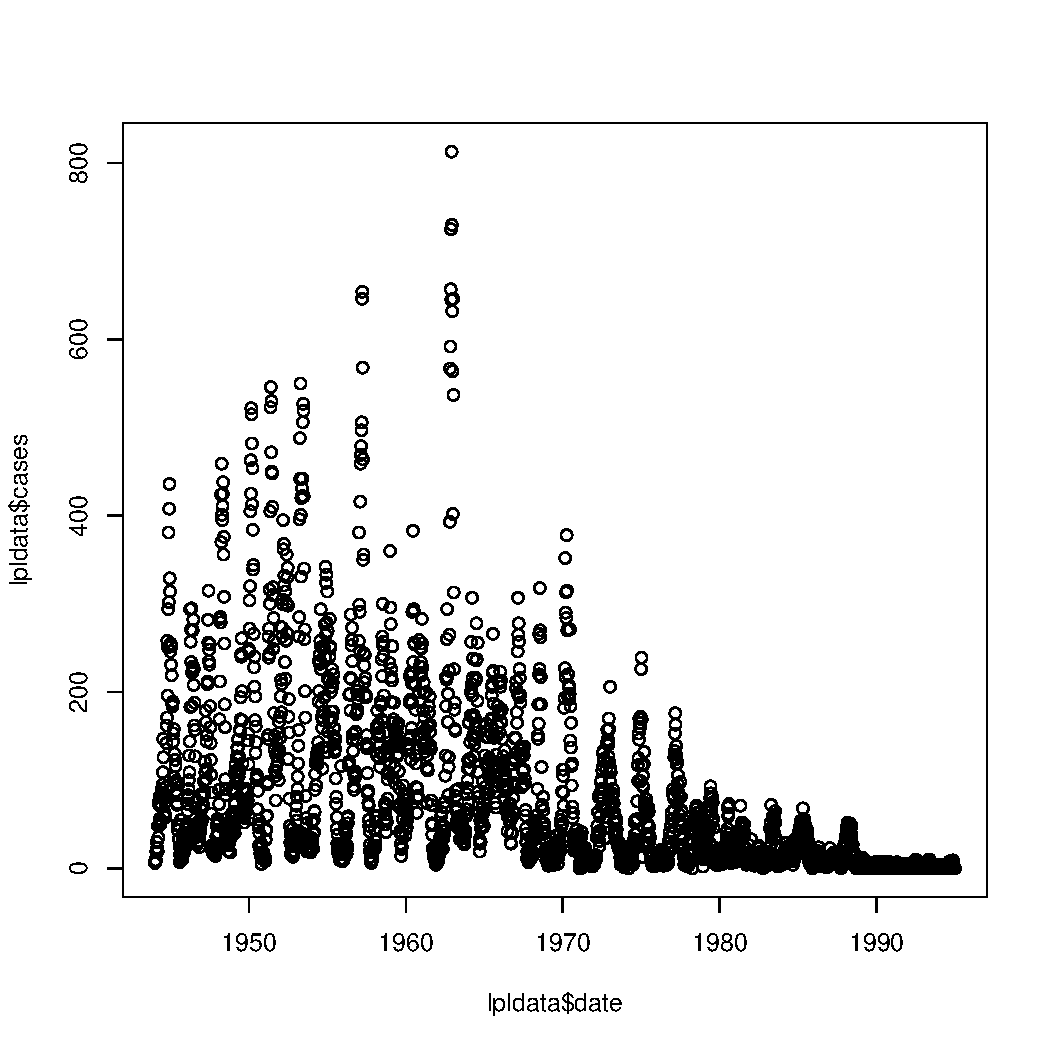
\includegraphics[width=\maxwidth]{figure/unnamed-chunk-5-1} 
\begin{kframe}\begin{alltt}
\hlkwd{par}\hlstd{(}\hlkwc{mfrow}\hlstd{=}\hlkwd{c}\hlstd{(}\hlnum{2}\hlstd{,}\hlnum{2}\hlstd{))} \hlcom{#create multiplot. two columns and two rows}

\hlcom{#periodogram of full time series}
\hlkwd{periodogram}\hlstd{(lpldata,}
            \hlkwc{main}\hlstd{=}\hlstr{"Entire timeseries"}\hlstd{,}
            \hlkwc{xlim}\hlstd{=}\hlkwd{c}\hlstd{(}\hlnum{0}\hlstd{,}\hlnum{300}\hlstd{),}\hlkwc{xlab}\hlstd{=}\hlstr{"Weeks"}\hlstd{,} \hlkwc{ylab}\hlstd{=}\hlstr{"Power"}\hlstd{)}
\hlkwd{periodogram}\hlstd{(londondata,}
            \hlkwc{end.date}\hlstd{=}\hlkwd{as.Date}\hlstd{(}\hlstr{'1950-01-01'}\hlstd{),}
            \hlkwc{xlim}\hlstd{=}\hlkwd{c}\hlstd{(}\hlnum{1}\hlstd{,}\hlnum{250}\hlstd{),}
            \hlkwc{main}\hlstd{=}\hlstr{"1944-01-07 to 1950-01-01"}\hlstd{,}
            \hlkwc{xlab}\hlstd{=}\hlstr{"Weeks"}\hlstd{,} \hlkwc{ylab}\hlstd{=}\hlstr{"Power"}\hlstd{)}

\hlcom{#strongest 2 year cycle. slightly less strong 1 year cycle}
\hlkwd{periodogram}\hlstd{(londondata,}\hlkwd{as.Date}\hlstd{(}\hlstr{'1950-01-01'}\hlstd{),}
            \hlkwd{as.Date}\hlstd{(}\hlstr{'1968-01-01'}\hlstd{),}
            \hlkwc{xlim}\hlstd{=}\hlkwd{c}\hlstd{(}\hlnum{1}\hlstd{,}\hlnum{250}\hlstd{),}
            \hlkwc{main}\hlstd{=}\hlstr{"1950-01-01 to 1968-01-01"}\hlstd{,}
            \hlkwc{xlab}\hlstd{=}\hlstr{"Weeks"}\hlstd{,} \hlkwc{ylab}\hlstd{=}\hlstr{"Power"}\hlstd{)}

\hlcom{#strong 3 year cycle. less strong 1 year cycle}
\hlkwd{periodogram}\hlstd{(londondata,}
            \hlkwd{as.Date}\hlstd{(}\hlstr{'1968-01-01'}\hlstd{),}
            \hlkwd{as.Date}\hlstd{(}\hlstr{'1994-12-31'}\hlstd{),}
            \hlkwc{xlim}\hlstd{=}\hlkwd{c}\hlstd{(}\hlnum{1}\hlstd{,}\hlnum{250}\hlstd{),}
            \hlkwc{main}\hlstd{=}\hlstr{"1968-01-01 to 1994-12-31"}\hlstd{,}
            \hlkwc{xlab}\hlstd{=}\hlstr{"Weeks"}\hlstd{,} \hlkwc{ylab}\hlstd{=}\hlstr{"Power"}\hlstd{)}
\end{alltt}
\end{kframe}
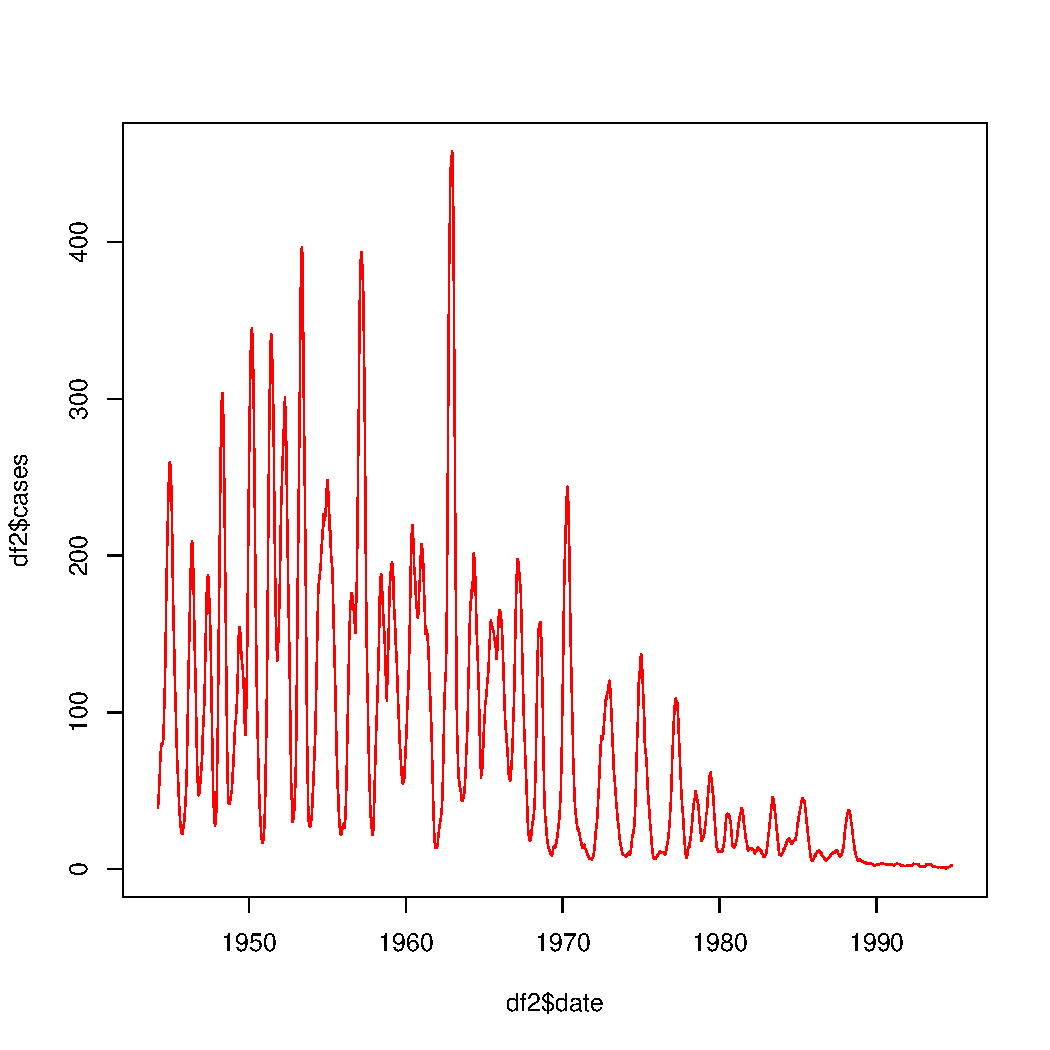
\includegraphics[width=\maxwidth]{figure/unnamed-chunk-5-2} 

\end{knitrout}

\end{enumerate}

\section{Stochastic Epidemic Simulations}

\SEintro

\begin{enumerate}[(a)]

\item \SEa

\begin{knitrout}
\definecolor{shadecolor}{rgb}{0.969, 0.969, 0.969}\color{fgcolor}\begin{kframe}
\begin{alltt}
\hlstd{SI.Gillespie} \hlkwb{<-} \hlkwa{function}\hlstd{(}\hlkwc{beta} \hlstd{=} \hlnum{1}\hlstd{,} \hlkwc{N} \hlstd{=} \hlnum{100}\hlstd{,} \hlkwc{I0} \hlstd{=} \hlnum{1}\hlstd{,} \hlkwc{tmax}\hlstd{=}\hlnum{10}\hlstd{) \{}

  \hlcom{# initialize variables}
  \hlstd{t} \hlkwb{<-} \hlnum{0}
  \hlstd{I} \hlkwb{<-} \hlstd{I0}
  \hlstd{S} \hlkwb{<-} \hlstd{N} \hlopt{-} \hlstd{I0}
  \hlstd{n} \hlkwb{<-} \hlnum{1}

  \hlkwa{while}\hlstd{(t[n]} \hlopt{<} \hlstd{tmax} \hlopt{&} \hlstd{I[n]} \hlopt{<} \hlstd{N) \{}
    \hlcom{# calculate event rate}
    \hlstd{a} \hlkwb{<-} \hlstd{beta}\hlopt{*}\hlstd{S[n]}\hlopt{*}\hlstd{I[n]}

    \hlcom{# generate uniform random variable}
    \hlstd{u} \hlkwb{<-} \hlkwd{runif}\hlstd{(}\hlnum{1}\hlstd{)}

    \hlcom{# time until next event}
    \hlstd{dt} \hlkwb{<-} \hlstd{(}\hlnum{1}\hlopt{/}\hlstd{a)}\hlopt{*}\hlkwd{log}\hlstd{(}\hlnum{1}\hlopt{/}\hlstd{(}\hlnum{1}\hlopt{-}\hlstd{u))}

    \hlcom{# record time}
    \hlstd{t[n} \hlopt{+} \hlnum{1}\hlstd{]} \hlkwb{<-} \hlstd{t[n]} \hlopt{+} \hlstd{dt}

    \hlcom{# update state}
    \hlstd{S[n}\hlopt{+} \hlnum{1}\hlstd{]} \hlkwb{<-} \hlstd{S[n]} \hlopt{-} \hlnum{1}
    \hlstd{I[n} \hlopt{+} \hlnum{1}\hlstd{]} \hlkwb{<-} \hlstd{I[n]} \hlopt{+} \hlnum{1}

    \hlcom{# increment counter}
    \hlstd{n} \hlkwb{<-} \hlstd{n}\hlopt{+}\hlnum{1}
  \hlstd{\}}

  \hlcom{# return time series}
  \hlkwd{tibble}\hlstd{(}
      \hlkwc{time} \hlstd{= t[}\hlnum{1}\hlopt{:}\hlstd{(}\hlkwd{length}\hlstd{(t)} \hlopt{-} \hlnum{1}\hlstd{)],}
      \hlkwc{infected} \hlstd{= I[}\hlnum{1}\hlopt{:}\hlstd{(}\hlkwd{length}\hlstd{(I)} \hlopt{-} \hlnum{1}\hlstd{)],}
      \hlkwc{susceptible} \hlstd{= S[}\hlnum{1}\hlopt{:}\hlstd{(}\hlkwd{length}\hlstd{(S)} \hlopt{-} \hlnum{1}\hlstd{)]}
  \hlstd{)}

\hlstd{\}}
\end{alltt}
\end{kframe}
\end{knitrout}

\item \SEb

\begin{knitrout}
\definecolor{shadecolor}{rgb}{0.969, 0.969, 0.969}\color{fgcolor}\begin{kframe}
\begin{alltt}
\hlkwd{library}\hlstd{(deSolve)}
\hlcom{# Function to describe }
\hlstd{SI.d} \hlkwb{<-} \hlkwa{function}\hlstd{(}\hlkwc{t}\hlstd{,} \hlkwc{y}\hlstd{,} \hlkwc{p}\hlstd{) \{}
  \hlkwd{with}\hlstd{(}\hlkwd{as.list}\hlstd{(}\hlkwd{c}\hlstd{(y, p)), \{}
    \hlstd{dI} \hlkwb{<-} \hlstd{beta}\hlopt{*}\hlstd{(N}\hlopt{-}\hlstd{I)}\hlopt{*}\hlstd{I}

    \hlkwd{return}\hlstd{(}\hlkwd{list}\hlstd{(}\hlkwd{c}\hlstd{(dI)))}
  \hlstd{\})}
\hlstd{\}}
\end{alltt}
\end{kframe}
\end{knitrout}

\begin{knitrout}
\definecolor{shadecolor}{rgb}{0.969, 0.969, 0.969}\color{fgcolor}\begin{kframe}
\begin{alltt}
\hlkwd{set.seed}\hlstd{(}\hlnum{8}\hlstd{)}
\hlstd{test.sizes} \hlkwb{<-} \hlkwd{tribble}\hlstd{(}
  \hlopt{~}\hlstd{pop,} \hlopt{~}\hlstd{tmax,}
  \hlnum{32}\hlstd{,} \hlnum{0.35}\hlstd{,}
  \hlnum{100}\hlstd{,} \hlnum{0.15}\hlstd{,}
  \hlnum{1000}\hlstd{,} \hlnum{0.02}\hlstd{,}
  \hlnum{10000}\hlstd{,} \hlnum{0.0025}
\hlstd{)}

\hlkwd{par}\hlstd{(}\hlkwc{mfrow} \hlstd{=} \hlkwd{c}\hlstd{(}\hlnum{2}\hlstd{,} \hlnum{2}\hlstd{))}

\hlstd{initial} \hlkwb{<-} \hlkwd{c}\hlstd{(}\hlkwc{I} \hlstd{=} \hlnum{1}\hlstd{)}


\hlkwa{for} \hlstd{(i} \hlkwa{in} \hlnum{1}\hlopt{:}\hlnum{4}\hlstd{) \{}
  \hlstd{size} \hlkwb{<-} \hlstd{test.sizes}\hlopt{$}\hlstd{pop[i]}
  \hlstd{tmax} \hlkwb{<-} \hlstd{test.sizes}\hlopt{$}\hlstd{tmax[i]}

  \hlstd{timesteps} \hlkwb{<-} \hlkwd{seq}\hlstd{(}\hlnum{0}\hlstd{, tmax,} \hlkwc{length.out} \hlstd{=} \hlnum{300}\hlstd{)}

  \hlstd{params} \hlkwb{<-} \hlkwd{c}\hlstd{(}\hlkwc{beta} \hlstd{=} \hlnum{1}\hlstd{,} \hlkwc{N} \hlstd{= size)}
  \hlstd{sol} \hlkwb{<-} \hlkwd{ode}\hlstd{(initial, timesteps, SI.d, params)}
  \hlkwd{plot}\hlstd{(}\hlkwd{as.data.frame}\hlstd{(sol),} \hlkwc{type} \hlstd{=} \hlstr{"l"}\hlstd{,} \hlkwc{lwd} \hlstd{=} \hlnum{3}\hlstd{,}
       \hlkwc{main}\hlstd{=} \hlkwd{str_c}\hlstd{(}\hlstr{"Solution of SI Model for N= "}\hlstd{, size))}

  \hlkwa{for} \hlstd{(j} \hlkwa{in} \hlnum{1}\hlopt{:}\hlnum{30}\hlstd{)\{}
    \hlkwd{lines}\hlstd{(}\hlkwd{SI.Gillespie}\hlstd{(}\hlkwc{beta} \hlstd{= params[}\hlstr{"beta"}\hlstd{],}
                       \hlkwc{N} \hlstd{= params[}\hlstr{"N"}\hlstd{],}
                       \hlkwc{I0} \hlstd{= initial[}\hlstr{"I"}\hlstd{],}
                       \hlkwc{tmax} \hlstd{= tmax),} \hlkwc{col} \hlstd{= j)}
  \hlstd{\}}
  \hlkwd{lines}\hlstd{(}\hlkwd{as.data.frame}\hlstd{(sol),} \hlkwc{type} \hlstd{=} \hlstr{"l"}\hlstd{,} \hlkwc{lwd} \hlstd{=} \hlnum{3}\hlstd{)}
\hlstd{\}}
\end{alltt}
\end{kframe}
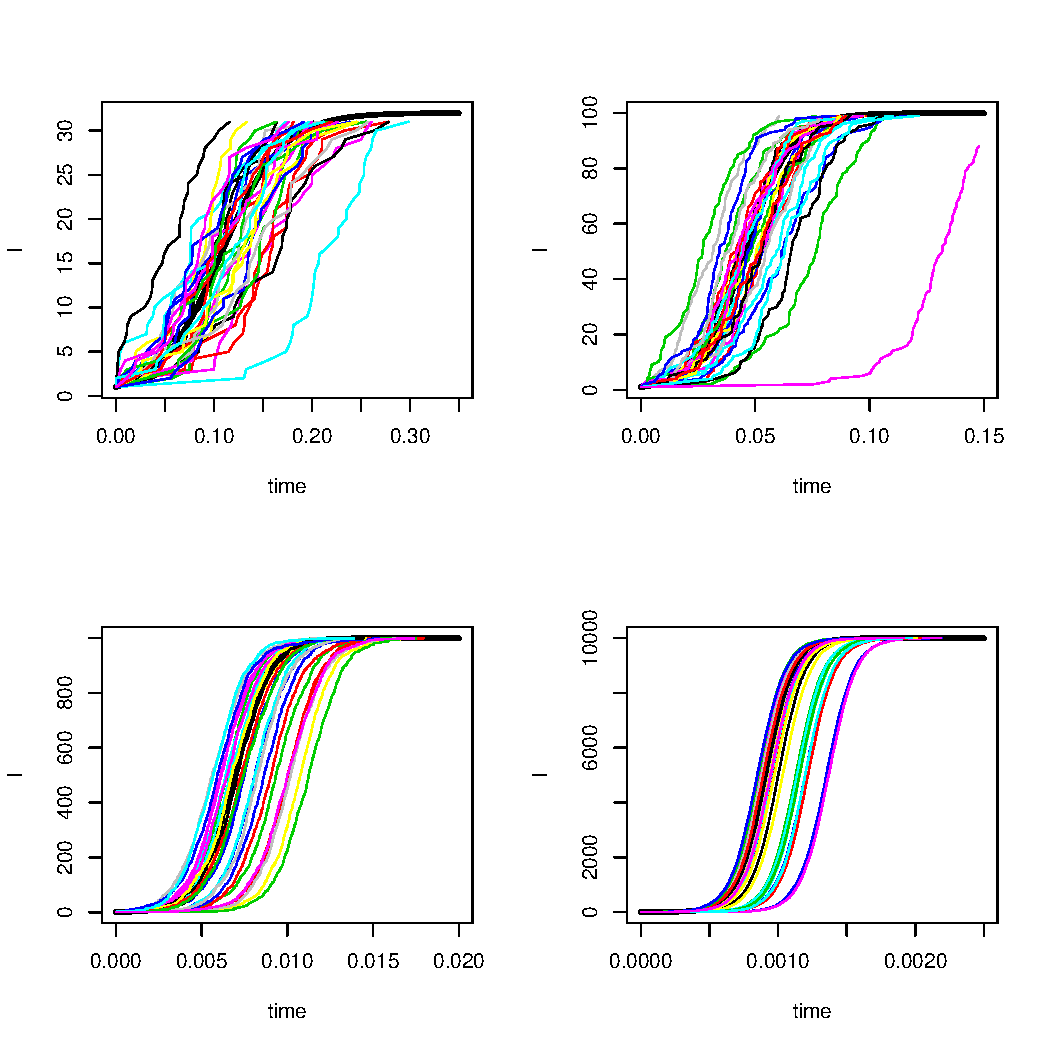
\includegraphics[width=\maxwidth]{figure/unnamed-chunk-8-1} 

\end{knitrout}

The Gillespie simulation was run 30 times for each of the 4 population sizes: N = 32 (top left), N = 100 (top right), N = 1000 (bottom left) and N = 10000 (bottom right). Different runs of the simulation are shown in different colors, while the deterministic solution (using the \texttt{deSolve} package) is shown with a thick black line. 

As $N$ increases, we see that the Gillespie simulation becomes smoother, and agrees more closely with the deterministic solution in shape. 

\end{enumerate}

\section{$\R_0$ for smallpox}

\Rintro

\begin{enumerate}[(a)]

  \item \Ra

    {\color{blue}{
Denote the susceptible state by $S$, the incubation state by $E$, and the recovered state by $R$. Furthermore, denote the four infectious stages by $I_1, I_2, I_3$, and $I_4$, respectively, and let the each of the stages represent the four different levels of infectiousness exhibited by infected individuals. For example, the $I_1$ stage corresponds to the prodrom stage, in which infectiousness is rare, while $I_4$ stage represents both the pustules \& scabs stage and the resolving scabs stage, as both of these stages share a low level of infectiousness. Note that all states are repsented by proportions.

Let $\sigma$ represent the per capita rate at which an infected individual develops symptoms and let $\gamma_i$ represent the per capita rate at which an infected individual in stage $i$ progresses to the next stage. In other words, $\gamma_i$ is considered to be the removal rate from stage $I_i$, such that the individual progresses to an infectiousness level exhibited in $I_{i+1}$. Moreover, note that $\gamma_4$ corresponds to the per capita recovery rate. 
Finally, let $\beta_i$ represent the infectiousness (per contact transmission rate) of an infected individual in stage $i$ and $\mu$ represent the per capita natural birth/death rate (they are assumed to be equal). Then, we can write an ODE model for this system as follows:
$$
\begin{aligned}
\frac{dS}{dt} &= \mu (1-S) - (\beta_1 I_1 + \beta_2 I_2 + \beta_3 I_3 + \beta_4 I_4) S\\
\frac{dE}{dt} &= (\beta_1 I_1 + \beta_2 I_2 + \beta_3 I_3 + \beta_4 I_4) S - (\sigma + \mu) E \\
\frac{dI_1}{dt} &= \sigma E - (\gamma_1 + \mu) I_1\\
\frac{dI_2}{dt} &= \gamma_1 I_1 - (\gamma_2 + \mu) I_1\\
\frac{dI_3}{dt} &= \gamma_2 I_2 - (\gamma_3 + \mu) I_1\\
\frac{dI_4}{dt} &= \gamma_3 I_3 - (\gamma_4 + \mu) I_1\\
\frac{dR}{dt} &= \gamma_1 I_4 - \mu R\\
\end{aligned}
$$
}}
  \item \Rb

{\color{blue}{
In order for an infected individual to infect a susceptible individual, it must survive the incubation period and become infectious. 
Then, we can think of $\R_0$ as the expected number of secondary cases caused by a typical infected individual, should they survive the incubation period and each of the following stages. This expression for $\R_0$ represents a sum of the basic reproductive numbers from each stage, such that the final number of secondary cases caused by the typical infective individual is merely equal to the number of infections they caused at each stage.
For example, the contribution of infection from the first stage would be equivalent to $\R_0$ of an SEIR model. We denote this value as $\R_{0,1}$:
$$
\beta_1 \times \frac{\sigma}{\sigma + \mu} \times \frac{1}{\gamma_1 + \mu}
$$
where $\beta_1/(\gamma_1 + \mu)$ represent the average number of infections that occur in stage 1 and $\sigma/(\sigma+\mu)$ is the probability that an infected individual does not die before the incubation period is over.
In order for infection to occur in stage $i>1$, an infected individual must not die from natural mortality before reaching stage $i$. Then, the contribution of infection during the second stage would be defined as $\R_{0,2}$, such that
$$
\beta_2 \times \frac{\sigma}{\sigma + \mu} \times \frac{\gamma_1}{\gamma_1 + \mu} \times \frac{1}{\gamma_2 + \mu}.
$$
Note that we now have $\gamma_1/(\gamma_1+\mu)$ to account for probability the of progressing to stage 2 without dying from natural causes while in stage 1.
Likewise, we can do a similar computation for all other stages. Summing each of our values for $\R_{0,i}$, we ultimately obtain
$$
\begin{aligned}
\R_0 &= \beta_1 \times \frac{\sigma}{\sigma + \mu} \times \frac{1}{\gamma_1 + \mu}\\
&+ \beta_2 \times \frac{\sigma}{\sigma + \mu} \times \frac{\gamma_1}{\gamma_1 + \mu} \times \frac{1}{\gamma_2 + \mu}\\
&+ \beta_3 \times \frac{\sigma}{\sigma + \mu} \times \frac{\gamma_1}{\gamma_1 + \mu} \times \frac{\gamma_2}{\gamma_2 + \mu} \times \frac{1}{\gamma_3 + \mu}\\
&+ \beta_4 \times \frac{\sigma}{\sigma + \mu} \times \frac{\gamma_1}{\gamma_1 + \mu} \times \frac{\gamma_2}{\gamma_2 + \mu} \times \frac{\gamma_3}{\gamma_3 + \mu} \times \frac{1}{\gamma_4 + \mu}.
\end{aligned}
$$
}}

  \item \Rc
{\color{blue} {
For this particular system, we have
$$
\mathcal{F} = \begin{pmatrix}
(\beta_1 I_1 + \beta_2 I_2 + \beta_3 I_3 + \beta_4 I_4) S\\
0\\
0\\
0\\
0
\end{pmatrix}, \mathcal{V} = \begin{pmatrix}
(\sigma + \mu) E \\
- \sigma E + (\gamma_1 + \mu) I_1\\
- \gamma_1 I_1 + (\gamma_2 + \mu) I_1\\
- \gamma_2 I_2 + (\gamma_3 + \mu) I_1\\
- \gamma_3 I_3 + (\gamma_4 + \mu) I_1\\
\end{pmatrix}
$$
Linearizing at the disease free equilibrium, we have
$$
F = \begin{pmatrix}
0 & \beta_1 & \beta_2 & \beta_3 & \beta_4\\
0 & 0 & 0 & 0 & 0\\
0 & 0 & 0 & 0 & 0\\
0 & 0 & 0 & 0 & 0\\
0 & 0 & 0 & 0 & 0\\
\end{pmatrix},
V = \begin{pmatrix}
(\sigma + \mu) & 0 & 0 & 0 & 0\\
- \sigma & \gamma_1 + \mu & 0 & 0 & 0\\
0 & - \gamma_1 & \gamma_2 + \mu & 0 & 0\\
0 & 0 & - \gamma_2 & \gamma_3 + \mu & 0\\
0 & 0 & 0 & - \gamma_3 & \gamma_4 + \mu\\
\end{pmatrix}
$$
Inverting matrix $V$ (by hand; steps not presnted), we observe:
$$
V^{-1} = \begin{pmatrix}
\frac{1}{\sigma + \mu} & 0 & 0 & 0 & 0\\
\frac{\sigma}{(\sigma + \mu)(\gamma_1 + \mu)} & \frac{1}{\gamma_1 + \mu} & 0 & 0 & 0\\
\frac{\sigma \gamma_1}{(\sigma + \mu)(\gamma_1 + \mu)(\gamma_2 + \mu)} & \frac{\gamma_1}{(\gamma_1 + \mu)(\gamma_2 + \mu)} & \frac{1}{\gamma_2 + \mu} & 0 & 0\\
\frac{\sigma \gamma_1 \gamma_2}{(\sigma + \mu)(\gamma_1 + \mu)(\gamma_2 + \mu)(\gamma_3 + \mu)} & \frac{\gamma_1 \gamma_2}{(\gamma_1 + \mu)(\gamma_2 + \mu)(\gamma_3 + \mu)} & \frac{\gamma_2}{(\gamma_2 + \mu)(\gamma_3 + \mu)} & \frac{1}{\gamma_3 + \mu} & 0\\
\frac{\sigma \gamma_1 \gamma_2 \gamma_3}{(\sigma + \mu)(\gamma_1 + \mu)(\gamma_2 + \mu)(\gamma_3 + \mu)(\gamma_4  +\mu)} & \frac{\gamma_1 \gamma_2 \gamma_3}{(\gamma_1 + \mu)(\gamma_2 + \mu)(\gamma_3 + \mu)(\gamma_4  +\mu)} & \frac{\gamma_2 \gamma_3}{(\gamma_2 + \mu)(\gamma_3 + \mu)(\gamma_4  +\mu)} & \frac{\gamma_3}{(\gamma_3 + \mu)(\gamma_4  +\mu)} & \frac{1}{\gamma_4  +\mu}\\
\end{pmatrix}
$$
It is clear that matrix $FV^{-1}$ consists of 0 entries except its first row.
Hence, its eigenvalues are on its diagonal, four of which are zero. The only non-zero entry on the diagonal is the first column entry of the first row, which is equal to the previously derived $\R_0$ value:
$$
\begin{aligned}
&\beta_1 \times \frac{\sigma}{\sigma + \mu} \times \frac{1}{\gamma_1 + \mu}\\
&+ \beta_2 \times \frac{\sigma}{\sigma + \mu} \times \frac{\gamma_1}{\gamma_1 + \mu} \times \frac{1}{\gamma_2 + \mu}\\
&+ \beta_3 \times \frac{\sigma}{\sigma + \mu} \times \frac{\gamma_1}{\gamma_1 + \mu} \times \frac{\gamma_2}{\gamma_2 + \mu} \times \frac{1}{\gamma_3 + \mu}\\
&+ \beta_4 \times \frac{\sigma}{\sigma + \mu} \times \frac{\gamma_1}{\gamma_1 + \mu} \times \frac{\gamma_2}{\gamma_2 + \mu} \times \frac{\gamma_3}{\gamma_3 + \mu} \times \frac{1}{\gamma_4 + \mu}\\
\end{aligned}
$$
Therefore, the derivation of $\R_0$ using the next generation method is consistent with the derivation of $\R_0$ from a biological argument.
}}

  \item \Rd

{\color{blue} {    
Note that for unaltered small pox, the time scale of disease is much shorter than average life span of a person. Then, we can approximate $\R_0$ by assuming that $\mu \approx 0$. The expression for $\R_0$ thus becomes
$$
\R_0 \approx \frac{\beta_1}{\gamma_1} + \frac{\beta_2}{\gamma_2} + \frac{\beta_3}{\gamma_3} + \frac{\beta_4}{\gamma_4}
$$
The alteration causes the early rash stage to be twice as long and so $\gamma_2^{-1}$ changes from 4 days to 8 days.
It is evident that increasing $\gamma_2^{-1}$ will lead to increase in $\R_0$.

Provided that infectiousness during the early rash stage is extreme, we can assume that at least half of the infection occurs during this stage. In the worst case scenario, all infections occur during the early rash stage. These assumptions are reasonable given that disease-induced death can occur in later stages, and so there would be little contribution to infection.
Based on these assumptions, we have that
$$
2.5 < \frac{\beta_2}{\gamma_{2,\tiny{\textrm{original}}}} < 5.
$$
Since altering doubles $\gamma_2^{-1}$, we get
$$
5 < \frac{\beta_2}{\gamma_{2,\tiny{\textrm{altered}}}} < 10.
$$
This translates to
$$
7.5 < \R_{0, \tiny{\textrm{altered}}} <10.
$$
}}
  \item \qRe

{\color{blue} {
We highly recommend that the CDC begin preparing for the smallpox attack immediately. Given that smallpox has been altered to have twice as long of an early rash stage, we expect $\R_0$ to increase by at least a factor of 1.5, and that is in the best-case scenario. In the worst case scenario, the $\R_0$ value corresponding to the altered smallpox will be twice as large as that of the unaltered smallpox, corresponding to the following range: $7.5 < \R_0 < 10$.
This means that the final size of an epidemic will be almost 100\% if the attack is successful.
}}

\end{enumerate}

\smpxnathistfig

\bigskip
\centerline{\bf--- END OF ASSIGNMENT ---}

\bigskip
Compile time for this document:
\today\ @ \thistime

\end{document}
